%!TEX root = main.tex
% \section{Motivations and Opportunities}
\section{Challeges and Motivations}
\label{sec:cam}
\subsection{Memory Imbalance in Pipeline Parallelism}
Pipeline parallelism is designed to distribute large model training across multiple devices
when a single device's memory cannot accommodate it.
However, significant memory inefficiency arises due to imbalanced memory usage across pipeline stages,
which contradicts its intended purpose.
To highlight this imbalance,
we conducted a benchmark test on the peak memory usage of each stage in GPipe and PipeDream.
The test was performed on a server with 8 A100 GPUs (40 GB each),
with pipeline stages set to 4 and 8 for GPipe and PipeDream, respectively.
\begin{figure*}[t]
  \centering
  \begin{minipage}[t]{0.33\linewidth}
    \centering
    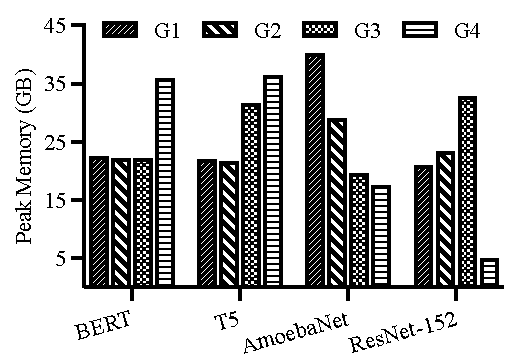
\includegraphics[width=0.95\linewidth]{GPipe-4GPUs.pdf}
    \caption{Peak Memory Usage of Each Stage on GPipe (4 GPUs)}
    \label{fig:gpipe-4gpus}
  \end{minipage}
  \begin{minipage}[t]{0.33\linewidth}
    \centering
    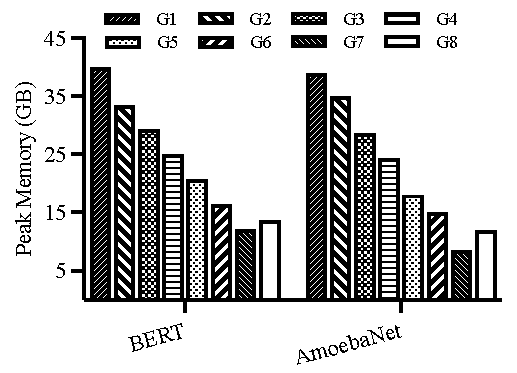
\includegraphics[width=0.95\linewidth]{PipeDream-8GPUs.pdf}
    \caption{Peak Memory Usage of Each Stage on PipeDream (8 GPUs)}
    \label{fig:pd-8gpus}
  \end{minipage}
  \begin{minipage}[t]{0.33\linewidth}
    \centering
    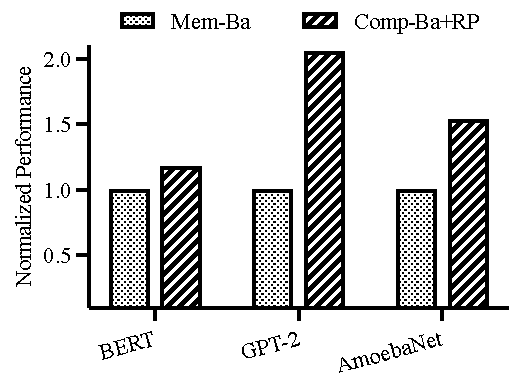
\includegraphics[width=0.95\linewidth]{normalized-perf.pdf}
    \caption{Normalized Performance of Two Different Partition Methods}
    \label{fig:norm-perf}
  \end{minipage}
\end{figure*}

Figure~\ref{fig:gpipe-4gpus} presents the benchmark results for GPipe, where G1 to G4 represent the GPU of different pipeline stages.
For the BERT model, the peak memory usage is nearly identical for the first three stages
but the last stage uses 13 GB more than the others.
This is because BERT, as a Transformer-based model with consistent computation and memory usage across its hidden layers,
shows balanced memory usage in the initial stages.
However, the last stage handles additional loss calculations and other post-processing functions,
leading to a significant memory spike.
A similar pattern is observed in T5, another Transformer-based model,
but with a peak memory shift to the third stage due to its encoder-decoder architecture.
In contrast, convolutional neural networks (CNNs) like ResNet-152 exhibit a different pattern.
Here, the ratio of computation times to memory usage varies with different types of layers.
For example, convolutional layers have longer computation times
while fully connected layers are more memory-intensive.
In ResNet-152, the last stage accounts for about 25\% of the total computation time but uses only 5 GB of memory,
creating a 27 GB difference compared to the third stage, which has the highest memory demand.
If peak memory usage across all stages is used as the baseline for GPU capacity,
this imbalance results in nearly 40\% and 34\% memory waste in ResNet-152 and AmoebaNet, respectively.

In synchronous pipeline parallelism,
memory imbalance across stages primarily arises from the uneven ratio
of computation time to memory usage among different layers in the model.
In asynchronous pipeline parallelism, this imbalance is further aggravated
by the varying number of copies of model parameters, activation memory, and gradients needed at each stage.
The benchmark result for PipeDream is shown in Figure~\ref{fig:pd-8gpus}.
The peak memory usage of the first stage reaches 40 GB,
while the smallest peak memory usage is only 12 GB in BERT.
In GPipe, the memory waste ratio for BERT is around 28\%, but in PipeDream, this waste ratio exceeds 40\%.
Furthermore, the memory waste ratio decreases by nearly 10\% compared to GPipe for AmoebaNet.
Whether using synchronous or asynchronous pipeline parallelism, significant GPU memory is wasted.
This memory waste limits the model size that can be accommodated to the stage with the highest memory usage,
despite substantial unused memory available on other GPUs.

\subsection{Computation Balance}
Based on the discussion above,
it is evident that focusing on balancing computation across pipeline stages
often leads to imbalanced memory usage, and vice versa.
Additionally, with memory optimization techniques like swapping and recomputation,
a key challenge arises when GPU memory is oversubscribed after partitioning a model for computational balance:
should the model be repartitioned to achieve more balanced memory usage,
or should memory optimization methods be applied to handle stages that exceed GPU capacity?
It’s difficult to determine which approach offers better training performance.
To explore this, we implemented two simple partitioning strategies in PipeDream for comparison.
The first method is memory-balanced partitioning (Mem-ba),
while the second combines compute-balanced partitioning with recomputation (Comp-ba+RP).
Both strategies achieve comparable maximum batch sizes,
and communication overhead does not significantly impact training performance.

The normalized performance results are shown in Figure~\ref{fig:norm-perf}.
Across all three models, the second method consistently outperforms the first,
particularly with the GPT-2 model,
where the training performance of Comp-Ba+RP is more than twice that of memory-balanced partitioning.
This performance gap is due to the significant difference in computation time between
the longest and shortest stages after memory-balanced partitioning in GPT-2.
Specifically, the computation time of the fourth stage reaches 286.275 ms
while the first stage only takes 29.104 ms — a nearly 10$\times$ difference.
As a result, the overall pipeline performance is severely constrained by the long computation time of the fourth stage.
Additionally, recomputation in GPT-2 provides significant memory savings with minimal additional computation overhead.
In the Comp-Ba+RP method, the total computation time for the fourth stage is reduced to 145.89 ms,
while the first stage, which requires more recomputation, increases to 136.89 ms.
This results in the fourth stage’s computation time being nearly halved compared to Mem-ba.
Similar improvements are observed in BERT and AmoebaNet, with performance gains of 1.18$\times$ and 1.54$\times$, respectively.
It is important to note that while the second method consistently outperforms in this benchmark,
this may not always hold true in every scenario.
The purpose of this section is to demonstrate that optimizing
pipeline parallel performance while considering memory limitations,
partitioning strategies, and memory optimization techniques is a complex and challenging problem.

\subsection{Motivation}
\label{sec:mot}
We observed that DL compilation techniques like XLA~\cite{sabneXlaCompilingMachine2020}
and TorchDynamo~\cite{anselPyTorchFasterMachine2024},
widely used in tensor parallelism for fine-grained analysis and automatic code generation,
have not been applied to pipeline parallelism in previous research.
Building on the fine-grained analysis provided by DL compilation,
we identified two key memory usage characteristics during model training that can guide pipeline partitioning.

First, most activation memory sizes are small,
making it easier to find low communication volumes between stages for efficient pipeline partitioning.
We profiled activation memory sizes for BERT, T5, GPT-2, and AmoebaNet, with results shown in Figure~\ref{fig:act-mem-cdf}.
In Transformer-based models, the largest activation memory is typically at the output layer,
which resides in the last stage and does not contribute to inter-stage communication.
For AmoebaNet, the largest activation memory (about 580 MB) comes from outputs of certain convolutional layers,
appearing only five times, so they are omitted in the figures. 
The data reveals that in GPT-2, T5, and AmoebaNet, over 90\% of computational nodes have activation memory sizes below 80 MB.
In T5, aside from the final output node, most activation memory is only around 50 MB.
In BERT, nodes with activation memory no greater than 128 MB account for over 80\% of the total nodes.
Even as batch size increases with pipeline partitioning, the communication overhead remains manageable.
For example, with four pipeline stages, a 4$\times$ transfer of 128 MB (512 MB total) over
a PCIe 3.0 $\times$16 link would take less than 40 ms, which is significantly shorter than the computation time.
\begin{figure}[htb]
  \centering
  \subfigure[Activation memory]{
    \centering
    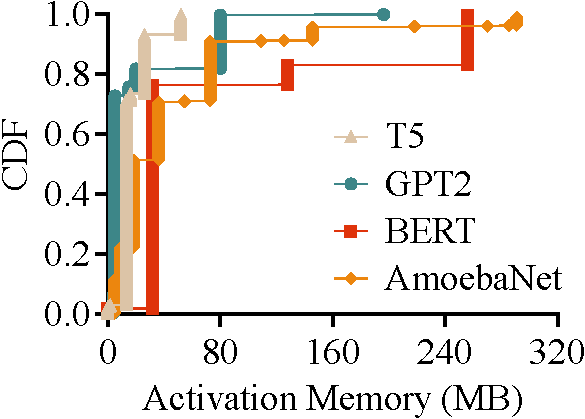
\includegraphics[width=0.47\linewidth]{act-mem-cdf-crop.pdf}
    \label{fig:act-mem-cdf}
  }
  \subfigure[Consumed Memory]{
    \centering
    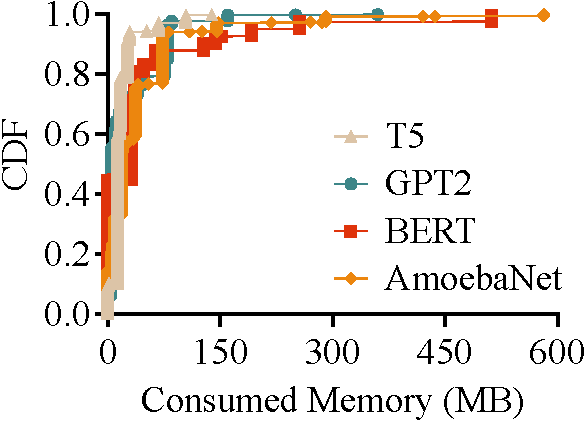
\includegraphics[width=0.47\linewidth]{consumed-mem-cdf-crop.pdf}
    \label{fig:cons-mem-cdf}
  }
  \caption{CDF of Node Activation Memory and Consumed Memory}
  \label{fig:mem-cdf}
\end{figure}

Secondly, the distribution of absolute memory consumption is shown in Figure~\ref{fig:cons-mem-cdf}.
Memory consumption here is calculated as the sum of memory allocated and released during node execution,
with released memory represented as a negative value.
The results show that in all four models, nearly 90\% of memory consumption per node is under 150 MB.
This suggests that partition points between stages can be flexibly adjusted between nodes with minimal memory usage,
allowing for small changes in the overall memory footprint of each stage while keeping communication overhead low.

Based on these insights, we propose a partitioning theorem for pipeline parallelism,
which will be discussed in detail in the next section.